

\subsection*{\Large Distance Measurement for changing Speed Setting}
    \begin{itemize}
        \item  Measuring distances with the robot is quite simple. But, what happens if the speed is changed?\\
        
        At higher speeds, number of measured distance points per time decrease and as expected, same distance would be covered in shorter time period.
       
       Let's see a case for two different speed settings: 28 and 50.\\ 
       This is done by changing the PWM values for each measurement.
            
\begin{lstlisting}[language=Python]

# Speed setting: 28, 50 \\Slower speeds for better measurement
SpeedArr = [28, 50];
    
def Robot_Meas(p):
    start = time.time()

    # threshold distance = 20cm, Max.distance = 1m
    while round(sensor.distance * 100, 2) > 20 and < 100:
        Time_Dist_Meas(start)
        Robot_Drive(p)  # Robot moves at given speed - 'p'

    end = time.time()
    Robot_STOP()
    
    # Loop using Speed Settings
for i in SpeedArr:
    filename = str(str(i) + '.txt') # file name using speed 
    print(filename)
    x = open(filename, 'w')
    TitleName(i)                # Title of text file

    led.on()
    Robot_Meas(i)
    led.off()

    # Manually return robot to original position
    time.sleep(5)  # Begin after 5s
    x.close()  # Close the file

\end{lstlisting}

\item The use of a certain distance ranges is to maintain accuracy in measurement and prevent crashing the robot.

\end{itemize}

\newpage

\begin{center}

    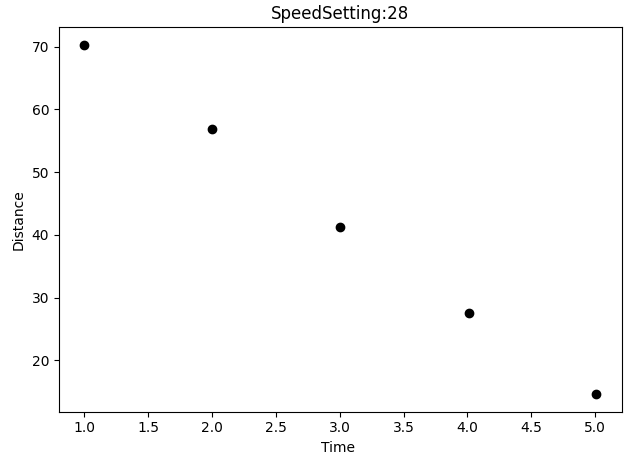
\includegraphics[width=0.7\textwidth]{./Speed_28}
    
    \vspace{1.5cm}
    
    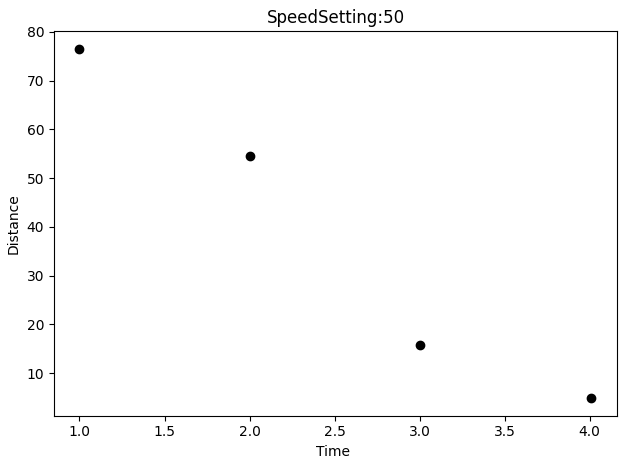
\includegraphics[width=0.7\textwidth]{./Speed_50}
\end{center}

